Our solution to automating several parts of the brewing system will require us to monitor and control the temperatures of the liquids inside of the HLT and the mash tun to the desired temperature that the brewer sets. Along with controlling the temperatures of the liquids, we will also control when liquid will be passed through the different kettles using pumps.

The main workhorse of the project will be the microcontrollers. We've chosen the ESP32 to be the main microcontroller in the project. The ESP32 will control heating the water in the hot liquor tank, which will pump the hot water from the HLT to the mashing tun for preheating. The microcontrollers will control the pumps and the heating elements as well.

\begin{figure}[H]
    \centering
    \graphicspath{.\images}
    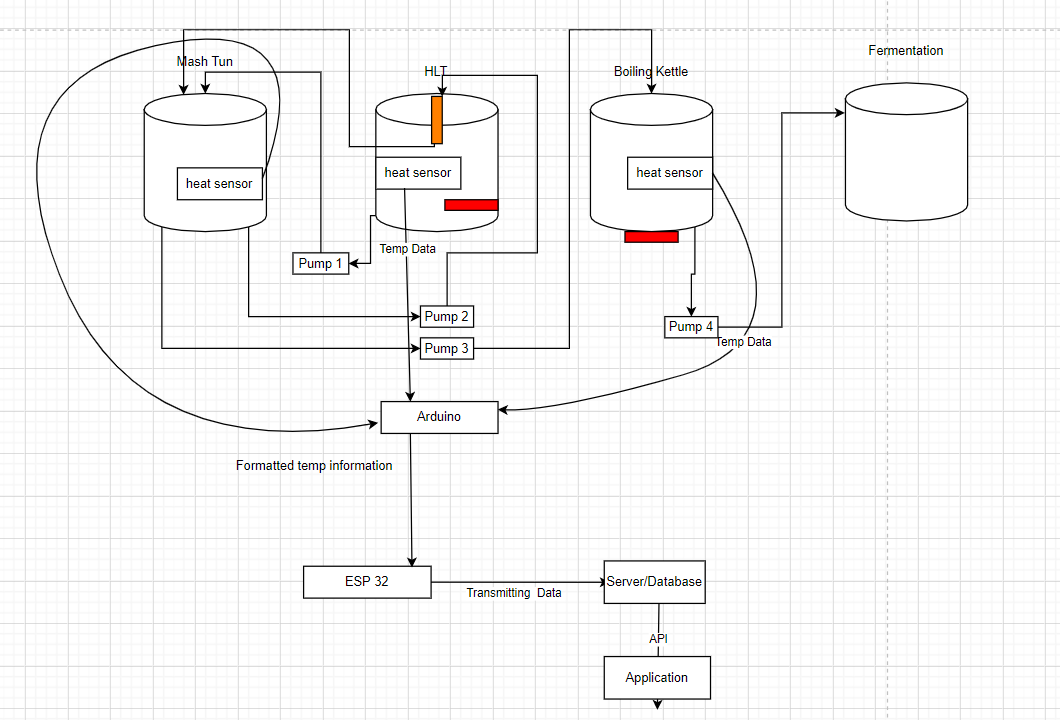
\includegraphics[scale=0.5]{images/sys_overview.PNG}
    \caption{System Overview}
\end{figure}

Equipment:
\begin{itemize}
	\item Four brewing kettles
	\item Three heat sensors
	\item Three pumps
	\item heating element
	\item heat exchanger coils
	\item microcontrollers/ESP32
	
\end{itemize}



